\chapter*{Введение}							% Заголовок
\addcontentsline{toc}{chapter}{Введение}	% Добавляем его в оглавление


\section*{Общие рассуждения}
Шагающие машины - это сложные системы с большим количеством степеней свободы и сложным управлением \cite{1984,2012}. Укажем, что для них центральной проблемой является синтез алгоритма управления. Большое количество внутренних степеней свободы предполагает нетривиальный подход к такому синтезу. 

Для дальнейшего важно сформулировать определение шагающей машины. Из многих существующих выберем следующее, основанное на основном свойстве такой машины оставлять дискретный след. Шагающая машина, - это машина, которая оставляет дискретный след на поверхности перемещения. Шагающий робот как автономная машина должен быть способен упорядоченным образом выбирать места для постановки опорных ног на поверхность.

Помимо алгоритмов управления при проектировании шагающих аппаратов возникает проблема выбора кинематической схемы аппарата и исполнительных механизмов двигательной системы. Возможные динамические нагрузки на аппарат вносят корректировки в выбор двигателей. Большой проблемой является соотношение скорости, мощности и массы. При помощи динамической модели можно достаточно хорошо оценить все параметры будущего робота правильно представлять возможности той или иной схемы или конструкции.


Большой интерес представляют задачи нетрадиционного передвижения шагающих аппаратов. Для передвижения по труднопроходимым областям отлично подходит ходьба, но на хорошо подготовленной поверхности, такой как дорога, преимущество на стороне колёсного транспорта. Отличным решением будет композиция качеств шагающего аппарата на труднопроходимой местности и колёсного аппарата на хорошей, подготовленной поверхности. При помощи небольшой модификации ног шагающего робота, можно добавить колёсный режим. В нужный момент, как только аппарат выбирается на хорошее покрытие, он становится на колёса и передвигается более быстро и эффективно. Возможны случаи, когда колёса не являются активными. Это значит, что в них нет движущих устройств, например электродвигателей, колеса могут свободно вращаться. В движение аппарат приводится за счёт специальных волнообразных движений ног, наподобие того, как разгоняются конькобежцы на роликовых или обычных коньках. Имеются публикации \cite{Roller-walker,Endo2000,GenEndo2012}.

Приведём примеры базовых кинематических схем ног аппарата, которые можно реализовать на базе унифицированных модулей, так называемых инсектоморфных ног.
На рис.\ref{fig1} приведена популярная базовая схема инсектоморфной ноги - ноги с тремя степенями свободы. Звенья лежат в одной вертикальной плоскости.

\begin{figure}[ht]
\center{\includegraphics[width=75mm]{Introduction/leg1}\\}
\caption{Три степени свободы}
\label{fig1}
\end{figure}

\begin{figure}[ht]
\center{\includegraphics[width=75mm]{Introduction/leg4}\\}
\caption{Четыре степени свободы}
\label{fig2}
\end{figure}

Инсектоморфная нога с одной дополнительной степенью свободы (всего их становится четыре) приведена на рис.\ref{fig2}. В схему ноги добавлен вращательный шарнир позволяющий поворачивать плоскость ноги вокруг звена длины $p_1$. Пара соседних ног с такой подвижностью может быть использована в качестве манипулятора\cite{Langosz2013,Roennau2013} и позволит роботу захватывать объекты, в то время как оставшиеся четыре ноги обеспечат роботу необходимую устойчивость.

\begin{figure}[ht]
\center{\includegraphics[width=75mm]{Introduction/leg5}\\}
\caption{Пять степеней свободы}
\label{fig3}
\end{figure} 

Инсектоморфная нога с двумя дополнительными степенями свободы приведена на рис.\ref{fig3}. Помимо дополнительного угла поворота плоскости ноги, в схеме имеется дополнительное звено на конце ноги. Угол поворота плоскости ноги и дополнительное звено позволят роботу ориентировать конец ноги под любым углом к контактной поверхности. Это может быть полезно в задачах по преодолению аппаратом различных препятствий и в задачах по манипуляции объектами сложной формы.

\begin{figure}
\begin{minipage}{0.49\linewidth}
\center{\includegraphics[width=75mm]{Introduction/leg2}\\ 1)}
\end{minipage}
\begin{minipage}{0.49\linewidth}
\center{\includegraphics[width=75mm]{Introduction/leg3}\\2)}
\end{minipage}
\caption{Колесно-шагающая схема и схема с зацепляющим устройством}
\label{fig4}
\label{fig5}
\end{figure}

Колёсно-шагающая конструкция ноги (рис. \ref{fig4}) позволяет переключаться из обычного режима ходьбы в колёсный режим. Колёса могут быть как пассивными, т.е. свободно вращающимися, так и активными, например с электромоторами. В пассивном колёсном режиме движение может осуществляться за счёт волнообразного движения колёс относительно контактной поверхности. 

Наконец, схема ноги со специальным устройством зацепления на конце ноги, позволяющим аппарату закрепляться на вертикальных поверхностях, показана на рис. \ref{fig5}. При синтезе шагового цикла для такой ноги необходимо учитывать принцип работы зацепного механизма ноги.

Отметим, что с развитием микроэлектроники большое распространение получил класс небольших шагающих роботов, так называемых мини-гексаподов, т.е. небольших шестиногих роботов. Это класс небольших и лёгких роботов, собранных в основном, на основе модельных серводвигателей, широко используемых в радиоуправляемых моделях самолётов, автомобилей, катеров, вертолётов и т.д. Эти роботы могут быть частично или полностью автономными, могут нести на себе сложную систему сенсоров и датчиков, производить все необходимые вычисления и обработку показаний сенсоров на бортовом вычислительном устройстве. Их кинематические схемы в основном следуют базовой схеме на рис. \ref{fig1}

\clearpage

\section*{О конструкциях шагающих машин. Обзор.}
Попытки создания шагающих машин уходят в глубокую древность. Однако, многие первые разработки были попытками имитировать или копировать ходьбу четвероногих животных. В литературных источниках (например, в Википедии) имеются указания, что одна из наиболее древних разработок датирована 230 BC (230 год до Рождества Христова) - деревянная лошадь с повозкой, автор Лю Бань, Китай. Современные репродукции деревянной лошади показаны на рис. \ref{fig6}

\begin{figure}[h]
\begin{minipage}{0.49\linewidth}
\center{\includegraphics[width=80mm]{intro1}}
\end{minipage}
\hfill
\begin{minipage}{0.49\linewidth}
\center{\includegraphics[width=80mm]{intro2}}
\end{minipage}
\caption{Схема одного из самых первых шагающих устройств}
\label{fig6}
\end{figure}

Разработки шагающих машин в дальнейшем прошли богатейшую историю. В современную историю одним из первых научной задачей анализа перемещения стопоходящих животных и устройств занялся известный русский математик и механик П.Л.Чебышев. Он в 1878 г. разработал образец так называемой стопоходящей машины \cite{..1945}, ее модель показана на рис. \ref{fig7}. Машина была построена на так называемых лямбда-механизмах Чебышева и была чисто механическим устройством. Стопоходящая машина является прекрасным примером его выдающихся работ по теории механизмов. 

\begin{figure}[here]
\center{\includegraphics[width=90mm]{intro3}}
\caption{Стопоходящая машина П.Л.Чебышева}
\label{fig7}
\end{figure}

Машина Чебышева показала принципиальную возможность создания шагающего устройства современными средствами. Однако в современном мире подобные устройства реализуются как роботы, в которых значительная часть или все функции управления реализуются бортовой автоматической (компьютерной) системой. При этом уже не требуется механическая связь движущихся ног и других частей аппарата, их заменяет логическая связь этих элементов в программе управления.


Первые пионерские работы по шагающим роботам в СССР были начаты в ИМАШ АН СССР, а затем их возглавил и стал бессменным лидером и руководителем академик РАН Д.Е. Охоцимский в ИПМ АН СССР (позднее ИПМ им.М.В.Келдыша РАН). Эти работы были на уровне передовых западных исследований, а во многом их опережали \cite{1984,1982,1972a,1978,1971,1974,1972,1974d,1977,1986b}.
Примерно в одно и то же время - в период 1972-1975 гг. - были созданы первые макеты многоногих шагающих машин. На рис.\ref{fig8} показан макет шагающей машины, разработанный в Институте машиноведения Академии наук СССР.

\begin{figure}[here]
\center{\includegraphics[width=90mm]{intro4}}
\caption{Шагающая машина ИМАШ РАН}
\label{fig8}
\end{figure}

В этой машине был использован оригинальный принцип организации ходьбы. Машина имеет 6 ног с так называемыми ортогональными приводами. Его преимущества состоят в более простых расчетных схемах синтеза движения ног и корпуса аппарата.
На рис.\ref{fig9} показаны макеты шестиногих шагающих машин, созданные в Институте прикладной математики АН СССР. Слева показан первый образец, созданный в содружестве ИПМ им. М.В.Келдыша АН СССР и Ленинградского механического института (ЛМИ), справа - второй образец, созданный несколько позднее при сотрудничестве ИПМ им. М.В.Келдыша АН СССР и Ленинградского института ВНИИТРАНСМАШ. 
Отметим, что эти аппараты имели так называемые инсектоморфные ноги, каждая из которых имела по три степени подвижности (три степени свободы). На рис.\ref{fig9} оба аппарата показаны в варианте с оснащением лазерным дальномерным устройством - Лазерным Измерителем Расстояний ЛИР. С помощью ЛИР роботы осматривали поверхность передвижения, и затем, управляющая роботами ЭВМ принимала решения о движении. Наличие шести ног позволяло решить принципиальную задачу устойчивости движения робота - робот мог передвигаться статически устойчивой походкой, если в каждый момент времени в опоре находилось не менее трех ног. Именно это обстоятельство определило интерес к многоногим машинам.

\begin{figure}[here]
\begin{minipage}{0.49\linewidth}
\center{\includegraphics[width=70mm]{intro5}}
\end{minipage}
\hfill
\begin{minipage}{0.49\linewidth}
\center{\includegraphics[width=70mm]{intro6}}
\end{minipage}
\caption{Шагающие роботы ИПМ им. М.В.Келдыша АН СССР. Фото 1975 г}
\label{fig9}
\end{figure} 

Позднее на базе этих разработок совместно ИПМ им. М.В.Келдыша АН СССР и ВНИИТРАНСМАШ в 1975 г. был создан большой натурный макет шестиногой машины НМША (Натурный Макет Шагающего Аппарата), которая была способна нести человека-оператора (водителя). Масса машины 750 кг. Скорость движения 0,7 км/ч, грузоподъёмность 50 кг, дорожный просвет 1,5 м. Машина показана на фотографиях на рис.\ref{fig10}.

\begin{figure}[h]
\begin{minipage}{0.49\linewidth}
\center{\includegraphics[width=70mm]{intro7}}
\end{minipage}
\hfill
\begin{minipage}{0.49\linewidth}
\center{\includegraphics[width=70mm]{intro8}}
\end{minipage}
\caption{Аппарат НМША}
\label{fig10}
\end{figure} 

Указанные исследования продолжаются в настоящее время, на рис.\ref{fig11} показан третий макет робота, создаваемый как модификация предыдущих в ИПМ им.М.В.Келдыша РАН. На роботе реализована оригинальная бортовая микропроцессорная система управления, построенная как бортовая микрокомпьютерная управляющая сеть. Робот оснащен необходимым набором сенсоров.

\begin{figure}[here]
\begin{minipage}{0.49\linewidth}
\center{\includegraphics[width=80mm]{intro9}}
\end{minipage}
\hfill
\begin{minipage}{0.49\linewidth}
\center{\includegraphics[width=80mm]{intro10}}
\end{minipage}
\caption{Шагающий робот ИПМ им. М.В.Келдыша РАН. 
Фотографии 2009 г}
\label{fig11}
\end{figure}
 
Работы по исследованию шестиногих аппаратов продолжаются и в МГУ, в Институте Механики. Они ведутся на основе модернизации самого первого проекта этого института, в котором создавался робот МАША (МАшина ШАгающая). 

\begin{figure}[here]
\begin{minipage}{0.49\linewidth}
\center{\includegraphics[width=80mm]{intro11}}
\end{minipage}
\hfill
\begin{minipage}{0.49\linewidth}
\center{\includegraphics[width=80mm]{intro12}}
\end{minipage}
\caption{Робот Института Механики МГУ. Первая (1975 г.) и современная версии}
\label{fig12}
\end{figure}
 
На рис.\ref{fig12} показана первая (слева) и современная (справа) версии робота МАША, на второй фотографии аппарат показан на переднем плане - на Фестивале мобильных роботов в МГУ. Робот также имеет шесть инсектоморфных ног и снабжен необходимым набором сенсоров.

Далее нужно отметить, что проекты шагающих машин выполнены практически во всех технологически развитых странах, - США, Японии, Англии, Финляндии, Бельгии, Германии, Испании, и других странах. Перечислим некоторые примеры. 

На рис.\ref{fig13} приведена одна из первых разработок в США. Авторы –Robert McGhee и Andrew Frank. Разработка была хорошо известна и получила в научно-популярной прессе шутливые прозвища Phoney Poney или ''Калифорнийская лошадь''.

\begin{figure}[h]
\center{\includegraphics[width=80mm]{intro13}}
\caption{1968 г. Phoney Poney. Калифорнийская лошадь}
\label{fig13}
\end{figure}

\begin{figure}[h]
\center{\includegraphics[width=80mm]{intro14}}
\caption{1969 г. GE Walking Truck. Ralph Mosher. США}
\label{fig14}
\end{figure}

На рис.\ref{fig14} - тяжелая шагающая машина General Electric, США. Управление ею было построено на основе копирующих автоматов, но человек, ведущий ее и руками и ногами, выдерживал всего порядка десяти минут. Такой сложной была система управления, требующая огромного напряжения внимания и сил. По этим результатам был сделан однозначный вывод: управление аппаратом необходимо переложить на компьютер. Все последующие аппараты строились как роботы с компьютерным управлением, реализующим больший или меньший объем функций управления в супервизорном или автономном режимах.

На последующих фотографиях на рис.\ref{fig15}- \ref{fig16} - разработки 70-80 годов ХХ века, затем более поздние и современные аппараты зарубежных лабораторий и фирм.

На рис.\ref{fig17} показана концепт-машина, созданная в Финляндии в фирме Plustech Oy Ltd. Машина предназначена для работы в лесу на лесоразработках, в условиях труднопроходимой местности с валунами, где не проходит тяжелая колесная и гусеничная техника.

\begin{figure}
\center{\includegraphics[width=90mm]{intro15}}
\caption{1976 г. Средний шестиногий робот. Университет Огайо. 
профессор R. McGhee. США}
\label{fig15}
\end{figure}

\begin{figure}
\begin{minipage}{0.49\linewidth}
\center{\includegraphics[width=80mm]{intro16}}
\end{minipage}
\hfill
\begin{minipage}{0.49\linewidth}
\center{\includegraphics[width=80mm]{intro17}}
\end{minipage}
\caption{1984 – 1991 гг. ASV. Тяжелый шестиногий аппарат. 
Университет Огайо, Стенфордский университет. США.
Руководитель разработки профессор K.J.Waldron}
\label{fig16}
\end{figure}



\begin{figure}[here]
\center{\includegraphics[width=90mm]{intro18}}
\caption{Plustech Oy Ltd. Финляндия, 1999}
\label{fig17}
\end{figure}

Далее – японские разработки (рис. \ref{fig18},\ref{fig19}), роботы семейства Titan. Масса робота Titan 11 составляет 7 тонн.

\begin{figure}[here]
\begin{minipage}{0.49\linewidth}
\center{\includegraphics[width=80mm]{intro19}}
\end{minipage}
\hfill
\begin{minipage}{0.49\linewidth}
\center{\includegraphics[width=80mm]{intro20}}
\end{minipage}
\caption{Titan 8. Япония. Лаборатория профессора Хиросе}
\label{fig18}
\end{figure}

\begin{figure}[here]
\center{\includegraphics[width=90mm]{intro21}}
\caption{Titan 11. Япония. Лаборатория профессора Хиросе}
\label{fig19}
\end{figure}

На рис.\ref{fig20} и рис.\ref{fig21} – разработки Германии и Испании, семейства средних роботов Lauron и Silo.

\begin{figure}[here]
\begin{minipage}{0.49\linewidth}
\center{\includegraphics[width=80mm]{intro22}}
\end{minipage}
\hfill
\begin{minipage}{0.49\linewidth}
\center{\includegraphics[width=80mm]{intro23}}
\end{minipage}
\caption{Lauron 3, Lauron 4. Германия}
\label{fig20}
\end{figure} 

\begin{figure}[here]
\begin{minipage}{0.49\linewidth}
\center{\includegraphics[width=80mm]{intro24}}
\end{minipage}
\hfill
\begin{minipage}{0.49\linewidth}
\center{\includegraphics[width=80mm]{intro25}}
\end{minipage}
\caption{Silo 4 (четырехногий) и Silo 6 (шестиногий). Испания}
\label{fig21}
\end{figure}
 
\clearpage

Наконец, на рис.\ref{fig22} – хорошо известные современные разработки фирмы Boston Dynamics, США, роботы Big Dog и Alpha Dog.

\begin{figure}[here]
\begin{minipage}{0.49\linewidth}
\center{\includegraphics[width=80mm]{intro26}}
\end{minipage}
\hfill
\begin{minipage}{0.49\linewidth}
\center{\includegraphics[width=80mm]{intro27}}
\end{minipage}
\caption{Роботы Big Dog (слева) и Alpha Dog}
\label{fig22}
\end{figure} 

%\clearpage

Сказанное о технологиях перехода к шагающим машинам как роботам с программным синтезом движения полностью подтверждается, например, работами по многоногим шагающим роботам в России в Волгоградском государственном техническом университете (ВолгГТУ). Здесь создаются машины с так называемыми цикловыми механизмами ходьбы и машины с оригинальными ортогональными приводами движителей. Образцом таких разработок может служить шагающая машина "Восьминог", показанная на рис.\ref{fig23}. В этой разработке механизмы шагания также построены на идее лямбда-механизма Чебышева, поэтому цикл шагания фактически создается механическим устройством ноги. Возможно, это несколько ограничивает адаптационные возможности машины, но ее бесспорным преимуществом является значительная простота системы управления и весьма высокая опорная проходимость машины. Машина способна двигаться и работать на очень слабых грунтах (рис. ~\ref{fig23}).

\begin{figure}[h]
\begin{minipage}{0.49\linewidth}
\center{\includegraphics[width=80mm]{intro28}}
\end{minipage}
\hfill
\begin{minipage}{0.49\linewidth}
\center{\includegraphics[width=80mm]{intro29}}
\end{minipage}
\caption{Машина "Восьминог" ВолгГТУ. Волгоград}
\label{fig23}
\end{figure} 

Однако, в дальнейшем авторы предприняли еще одно направление работ – создание машин с ортогональными шагающими движителями. На рис.\ref{fig24} показан средний макет восьминогого робота с ортогональными приводами (характерный размер машины – 1 м). Движитель организован как два модуля с четырьмя опорами каждый и для реализации поворота машины модули могут поворачиваться друг относительно друга. Наличие в аппарате большого числа степеней свободы приводит к необходимости бортового компьютерного управления этой машиной. Система управления для этой машины разрабатывается в ИПМ им. М.В.Келдыша РАН.

\begin{figure}[here]
\center{\includegraphics[width=90mm]{intro30}}
\caption{Робот с ортогонально-поворотным движителем. ВолгГТУ. Волгоград}
\label{fig24}
\end{figure}
\begin{figure}[here]
\center{\includegraphics[width=90mm]{intro31}}
\caption{Шагающая машина "Ортоног". Волгоград}
\label{fig25}
\end{figure} 

Как развитие этих исследований в ВолГТУ выполняется проект по созданию большой шагающей машины с 4-мя спаренными ортогонально-поворотными движителями, общим весом 2 т и грузоподъемностью до 1 т (рис.\ref{fig25}). В настоящее время завершено изготовление машины, начаты интенсивные работы по программированию ее системы управления. Укажем некоторые важные проекты мини-гексаподов. Они приведены на рис.\ref{fig26} и рис.\ref{fig27}.

\begin{figure}[here]
\begin{minipage}{0.49\linewidth}
\center{\includegraphics[width=70mm]{intro38}}
\end{minipage}
\hfill
\begin{minipage}{0.49\linewidth}
\center{\includegraphics[width=70mm]{intro39}}
\end{minipage}
\caption{Lynxmotion (слева) и MSR-H01-01(справа)}
\label{fig26}
\end{figure} 

\begin{figure}[here]
\begin{minipage}{0.49\linewidth}
\center{\includegraphics[width=70mm]{intro40}}
\end{minipage}
\hfill
\begin{minipage}{0.49\linewidth}
\center{\includegraphics[width=70mm]{intro41}}
\end{minipage}
\caption{ARTEX (слева) и MORPHEX (справа)}
\label{fig27}
\end{figure}

Нетрудно заметить, что все это небольшие машины (размер в поперечнике меньше 0.5 м), достаточно легкие, предназначенные главным образом для исследований проблем шагающего движения. На проект робота MORPHEX (рис. ~\ref{fig27}) следует обратить особое внимание - это робот-трансформер, который способен принимать шарообразную форму и катиться по поверхности. При необходимости он снова раскрывается в шестиногий аппарат.

Анализируя приведенные обзорные данные, отметим с одной стороны удивительную кинематическую схожесть различных проектов, выполненных в разных лабораториях. Можно считать, что сформировались несколько типовых классов шагающих машин – основные из них, это малые, до 0.5 м, средние, порядка 1 м, и большие роботы.


\newpage
\subsection*{Этапы создания шагающей машины}
Одним из первых этапов в проектировании шагающего робота является выбор конструкции и кинематики ноги и определение числа ног машины. Оптимальное количество ног (и их конструкция) определяются назначением шагающей машины (ШМ) и средой ее применения. 
Число ног, равное шести, является оптимальным с точки зрения наибольшей свободы и скорости передвижения в рамках статической устойчивости. 

\emph{Четырехногая} ШМ обычно имеет меньшие габариты, вес и более простую конструкцию, она также может двигаться в рамках статической устойчивости. Но ее профильная и опорная проходимость меньше, чем у шестиногой, скорость движения также меньше при прочих равных условиях.

\emph{Двуногая} машина может иметь самые малые размеры, но ее движение возможно только в рамках динамической устойчивости, организация такого движения весьма сложна. 

\emph{Многоногие} машины имеют большую грузоподъемность при заданных ограничениях давления на грунт и размер стоп. 
Говоря о кинематике ноги, укажем основные биологические прототипы. Они показаны на рис. \ref{fig28}. Среди всего разнообразия в живой природе наибольший интерес как основные прототипы представляют конечности насекомых и рептилий (первый рисунок на рис.\ref{fig28}), млекопитающих (средний рисунок), птиц (правый рисунок).


%\begin{figure}[here]
%\begin{minipage}{0.40\linewidth}
%\center{\includegraphics[width=30mm]{intro32}}
%\end{minipage}
%\hfill
%\begin{minipage}{0.40\linewidth}
%\center{\includegraphics[width=30mm]{intro33}}
%\end{minipage}
%\hfill
%\begin{minipage}{0.40\linewidth}
%\center{\includegraphics[width=30mm]{intro34}}
%\end{minipage}
%\caption{Ноги биологических существ-прототипов}
%\label{fig26}
%\end{figure}


\begin{figure}[here]
\center{\includegraphics[width=150mm]{intro32-34}}
\caption{Ноги биологических существ-прототипов}
\label{fig28}
\end{figure}

История и примеры развития шагающих машин таковы, что наибольший интерес у разработчиков вызывала и вызывает первая схема – так называемые инсектоморфные (насекомоподобные) ноги. Этот вариант реализовывался в подавляющем большинстве конструкций. На рис.\ref{fig29} показана типичная схема и конструкция такой ноги с 5-ю степенями подвижности.
После выбора схемы шагающего движителя возникают общие вопросы выбора компоновки, системы управления, сенсоров, программного обеспечения робота.
\begin{figure}[here]
\begin{minipage}{0.49\linewidth}
\center{\includegraphics[width=50mm]{intro35}}
\end{minipage}
\hfill
\begin{minipage}{0.49\linewidth}
\center{\includegraphics[width=50mm]{intro36}}
\end{minipage}
\caption{Инсектоморфная конечность}
\label{fig29}
\end{figure}

\begin{figure}[here]
\center{\includegraphics[width=110mm]{intro37}}
\caption{Этапы проекта шагающей машины}
\label{fig30}
\end{figure} 

Соответствующая общая схема этапов проектирования ШМ приведена на рис.\ref{fig30}.

В заключение этого обзора, подведем итог. Шагающий способ представляет основной интерес для движения по заранее неподготовленной местности с препятствиями. Традиционные колесные и гусеничные транспортные машины оставляют за собой непрерывную колею, а в случае передвижения шагами, взаимодействие с грунтом происходит только в местах опоры стопы. При шагающем способе меньше разрушается грунт, что, например, важно в тундре. Помимо этого шагающий способ передвижения обладает и большей специфической проходимостью на пересеченной местности вплоть до возможности передвигаться прыжками и т.п. При движении по достаточно гладким и подготовленным поверхностям способ перемещения при помощи шагания уступает колесному в экономичности, скорости передвижения и простоте управления.
Отмечая проблемы, решение которых не завершено, укажем следующие. Одной из проблем, которой уделяется существенное внимание при проектировании мобильных шагающих аппаратов, является уменьшение необходимой мощности источников питания и сокращение затрат энергии. Необходимо повысить к.п.д. многоногих механизмов, т.е. уменьшить потребляемую мощность и повысить развиваемую мощность. В самом деле, если учесть, что в общем случае каждая из конечностей имеет две-три-четыре степени подвижности и управление каждой из степеней сопряжено с определенными затратами энергии, то очевидно, что сравнение шагающих и колесных транспортных средств по к.П.Д. будет не в пользу первых. В связи с этим важная цель, к достижению которой должны стремиться исследователи сегодня, заключается в создании экспериментальных шагающих аппаратов, способных на практике продемонстрировать сочетание высоких функциональных возможностей с достаточно большой развиваемой мощностью при сниженных затратах энергии. Возможно, это потребует создания новых приводов для ШМ.
Отдельное важнейшее направление – создание новых перспективных планетных роверов. Следует добавить, что, по всей вероятности, эти потребности будут удовлетворяться, прежде всего, за счет шагающих аппаратов с шестью конечностями.

\subsection*{Современное состояние}
Много кто способен сейчас сделать робота буквально на коленке. Управляющая электроника и необходимые двигатели стали доступней в последнее время. Обычный человек может получить доступ к самым современных технологиям производства, таким как лазерная резка или 3d печать деталей из пластика. Современные САПР (Система Автоматизированного Проектирования) комплексы позволяют получить прототип детали в считанные часы. Стоимость комплектующих постоянно уменьшается, а качество и мощность постоянно растут. Всё это понижает входной порог в современной робототехнике. В сети интернет публикуется большое количество работ от энтузиастов одиночек, которые увлекаются созданием различных устройств и роботов. Не нужно отдельное конструкторское бюро и заводские условия чтобы создавать роботов в наши дни. Достаточно заказать подходящую электронику по интернету и напечатать механику на 3d принтере или вырезать лазером из листового металла необходимые детали и робот готов. Не все детали можно напечатать на 3d принтере, некоторые придётся изготовить обычным методом, на токарном или фрезерном станке, но можно упростить себе задачу и заказывать через интернет.

Робототехника получает второе дыхание. Лет сорок назад людям казалось, что пройдёт всего каких-то лет 30-40 и будет создан искусственный интеллект и роботы будут повседневным атрибутом нашей жизни. Роботам можно будет поручить рутинную, опасную работу, а человеку останется много свободного времени. В чём-то прогнозы сбылись, современные автоматизированные производственные линии значительно повысили эффективность труда, там, где раньше работали десятки токарей, теперь достаточно поставить один обрабатывающий центр и он будет работать круглосуточно, без больничных и отпусков.

Все это не совсем робототехника, это просто сложные автоматы, созданные людьми. Станки принципиально не изменились, произошла замена электроники и двигателей. Всё так же далеко до создания искусственного интеллекта, как и 30-40 лет назад. Подавляющее большинство роботов годится только для лабораторного использования, по-настоящему способных работать в человеческой среде аппаратов очень мало. Не всё так плохо, тенденция к появлению автономных аппаратов способных работать в неподготовленных условиях определенно наблюдается. Значительного успеха в этой области достигла американская компания Boston Dynamics. Первый значительный успех произошёл в 2005 году, когда публике был представлен робот BigDog \cite{BigDog}. 

\begin{figure}[t]
\center{\includegraphics[width=100mm]{BigDog_Snow}}
\caption{BigDog}
\end{figure}

BigDog — четырёхногий робот с адаптивным управлением, созданный в 2005 году фирмой Boston Dynamics совместно с Foster-Miller, Лабораторией реактивного движения (NASA) и Harvard University Concord Field Station.

Проект BigDog финансируется агентством перспективных военных разработок (Defense Advanced Research Projects Agency, DARPA) с надеждой на то, что он сможет переносить снаряжение и помогать солдатам на территории, где не способен передвигаться обычный транспорт. Вместо колёс и гусениц BigDog использует четыре ноги. В ногах находится большое количество разнообразных сенсоров. Также у BigDog имеется лазерный гироскоп и система бинокулярного зрения.
Длина робота BigDog — 0,91 метр, высота 0,76 метра, вес 110 килограммов. В настоящее время он способен передвигаться по труднопроходимой местности со скоростью 6,4 км в час, перевозить 154 кг груза и подниматься на 35 градусную наклонную плоскость. Его передвижение контролирует компьютерная система, которая получает данные от различных сенсоров. Навигация и равновесие также управляются этой системой.
BigDog упоминается в статьях New Scientist, Popular Science, Popular Mechanics и Wall Street Journal, а также в нескольких видео на сайте Youtube.
18 марта 2008 года Boston Dynamics выпустила видео о новом поколении робота BigDog. Видео показывает возможность робота ходить по ледяной поверхности и возможность восстанавливать равновесие после удара сбоку.

BigDog приводится в движение двухтактным одноцилиндровым двигателем от карта со скоростью вращения 9000 об/мин, из-за чего слышен громкий звук мотора. В последующих версиях робота планируется исправить этот демаскирующий недостаток. Мотор служит приводом для гидронасоса, который в свою очередь питает гидравлику ног. В каждой из ног установлено по 4 гидравлических привода (два для бедренного сустава, и по одному для коленного и голеностопного суставов) общим числом 16. Каждый из гидравлических двигателей состоит из гидроцилиндра, сервоклапана, а также датчиков положения и усилия. Робот обладает хорошей устойчивостью: во время испытаний он не падал при проходе по льду и при сильных толчках.
Бортовой компьютер робота представляет собой упрочненный вариант платформы PC/104 с процессором класса Pentium под управлением ОС QNX.

В 2012 году была представлена новая версия аппарата, получившая название Legged Squad Suppor System(LS3)\cite{LS3}. Новая версия аппарата отличается большей грузоподъёмностью и возможностью работать в сложных условиях.
\begin{figure}
\center{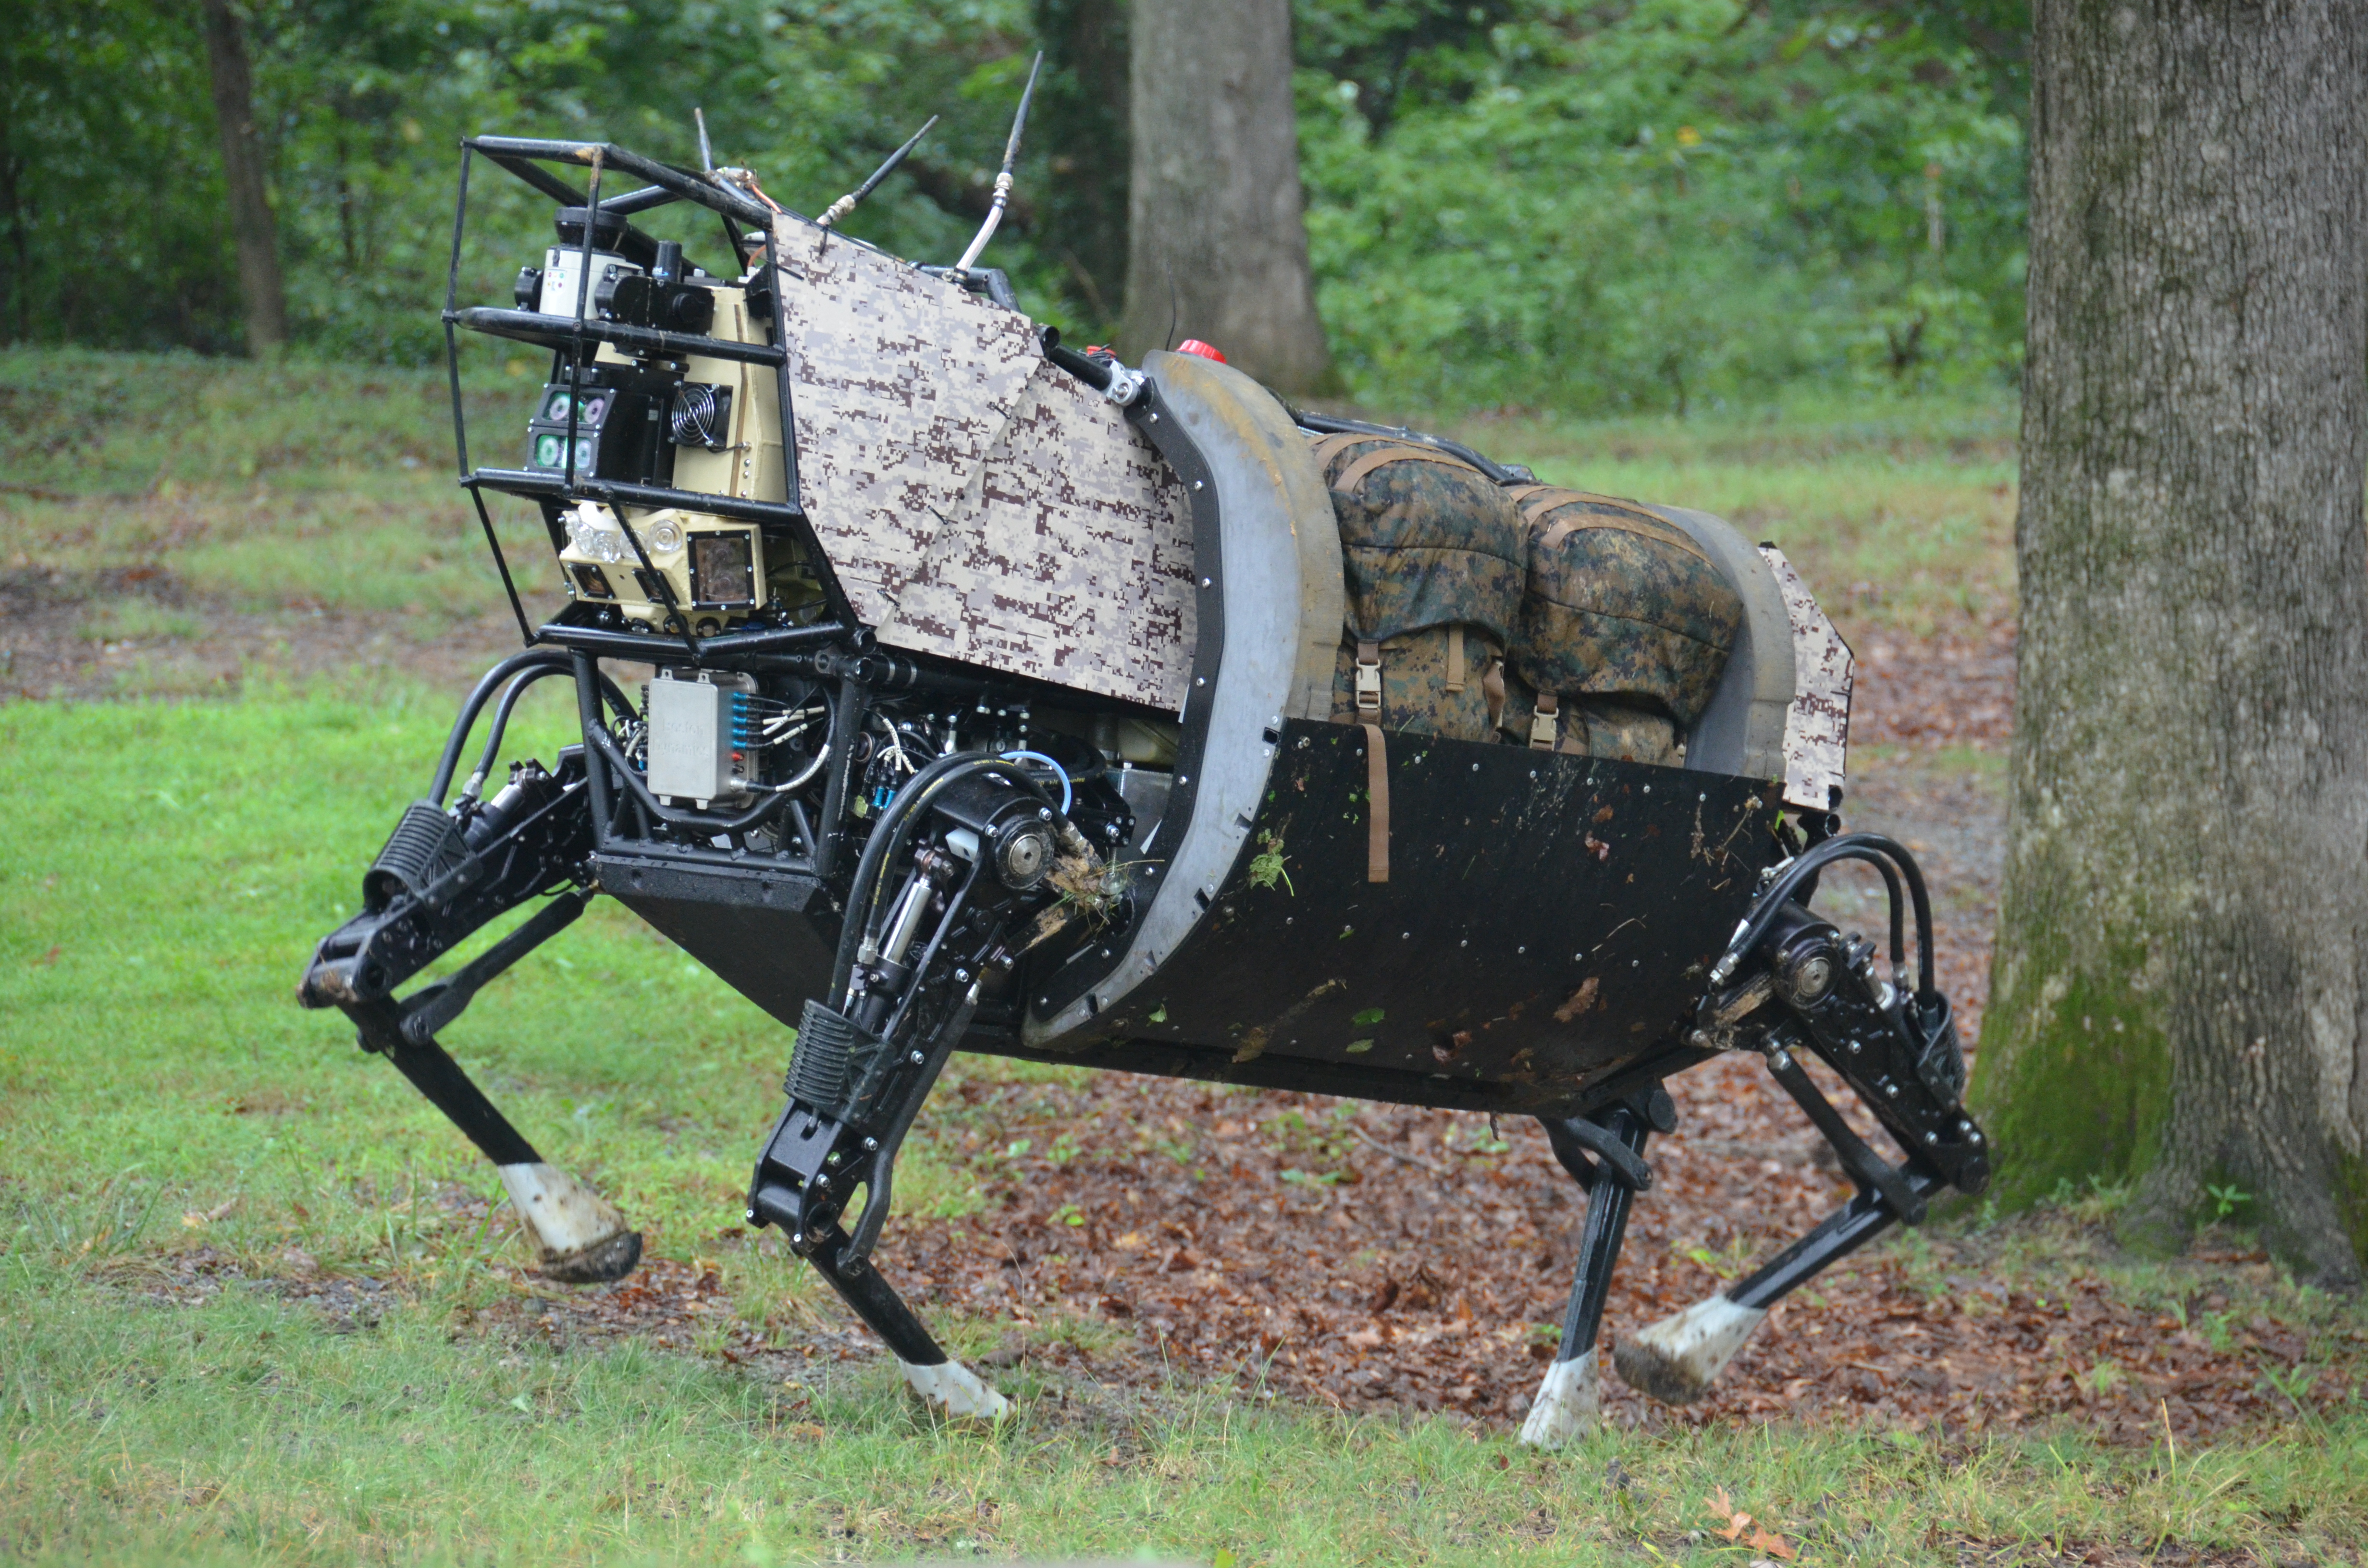
\includegraphics[width=100mm]{DSC_0502}}
\caption{Legged Squad Support System - LS3}
\end{figure}

Аппарат способен нести до 180кг нагрузки, преодолевать пересеченную местность, быстро реагировать и работать в тихом, беззвучном режиме, когда это необходимо. Система стереозрения, установленная в передней части аппарата, позволяет распознавать ведущего и следовать за ним в автоматическом режиме. Добавлена опция восприятия голосовых команд. Доработаны алгоритмы ходьбы по сложной, каменистой местности, доработан переход на трусцу и бег на ровных поверхностях. Планируется поставить первые серийные системы LS3 в действующие отряды морской пехоты США к 2014 году.


Шестиногие аппараты относятся к классу статически устойчивых аппаратов. Шестиногие роботы могут передвигаться, сохраняя статическую устойчивость. Это следует из того, что для шестиногого аппарата существуют классы походок, для которых верно, что в каждый момент времени три ноги аппарата находятся в опорной фазе и проекция центра масс робота попадает во внутреннюю область опорного треугольника. Среди аппаратов подобного класса широко известно семейство аппаратов Lauron и шагающее шестиногое шасси Mantis компании Micromagic Systems.


\begin{figure}[h]
\begin{minipage}[h]{0.49\linewidth}
\center{\includegraphics[width=80mm]{800px-Lauron4c_2009_FZI_Karlsruhe}}
\caption{LAURON IV}
\end{minipage}
\begin{minipage}[h]{0.49\linewidth}
\center{\includegraphics[width=80mm]{8586212180_99ffd2e15e}}
\caption{Carausius morosus}
\end{minipage}
\end{figure}


LAURON --- шестиногий шагающий робот, который разрабатывается в Исследовательском Центре Информационных Технологий (FZI) в Карлсруэ, Германия. Робот являются имитацией реального насекомого Carausius Morosus из семейства палочных насекомых. Создание шагающего робота началось с фундаментального исследования в области шестиногой ходьбы в начале 1990-х годов и привело к созданию первых роботов, названных Lauron. В 1994 году первый робот был представлен публике на выставке CeBIT в Ганновере. Стоит отметить, что разработки  по шестиногим шагающим аппаратам велись в ИПМ имени М.В. Келдыша ещё в 70-80 годы.

Первое поколение Lauron, в отличие от более поздних версий, управлялось при помощи искусственной нейронной сети. Именно поэтому первый робот получил название LAURON. От немецкого - LAUfROboter Neuronal gesteuert (English: Walking Robot, Neural Controlled).

\begin{figure}
\center{\includegraphics[width=80mm]{LAURON_V_-_2013_FZI_Karlsruhe}}
\caption{LAURON V}
\end{figure}

Самая последняя версия семейства LAURON была представлена в 2013 году, на Международной Конференции по Робототехнике и Автоматизации (ICRA), в Карлсруэ, Германия. Кинематика робота была улучшена, путём добавления дополнительного вращательного шарнира в бедренный сустав каждой ноги \cite{Roennau2013}. Такая модификация позволит роботу всегда держать плоскость ноги в вертикальном положении, что снижает нагрузку на шарниры ног при движении по крутому склону насыпи. Так же, дополнительная степень свободы теперь позволяет аппарату выполнять различные манипуляции с объектами, используя пару передних ног как пару манипуляторов. 

Аналогичный проект шагающего шестиногого аппарата \cite{Langosz2013} ведёт Центр Инновационной Робототехники (Robotics Innovation Center) под эгидой Немецкого Исследовательского Центра Искусственного Интеллекта (DFKI GmbH), город Бремен, Германия. 

\begin{figure}[h]
\center{\includegraphics[width=100mm]{20110225_SpaceClimber_Cebit_Foerderer}}
\caption{Space Climber}
\end{figure}

Цель программы SpaceClimber состоит в разработке аппарата с инсектоморфной (насекомоподобной) кинематикой \cite{1984}, способного энергетически эффективно преодолевать крутые склоны. Предполагается, что аппарат будет автономно исследовать внеземные кратеры, например, на Луне или Марсе. Аппарат будет доставляться в зону исследования на планетоходе и выгружаться при помощи специального крана-манипулятора установленного на ровере. Планетоход так же разрабатывается в Центре Инновационной Робототехники. Проект находится на стадии испытаний, на специальном лунном полигоне, имитирующем склоны лунных кратеров. По итогам программы планируется получить подтверждение, что шагающие аппараты являются основным инструментом в вопросе исследований труднопроходимых поверхностей, кратеров, расщелин и т.д.

 Компания Micromagic Systems основана в 1999 году и занимается разработкой аниматронов - роботов для создания анимированных персонажей и спецэффектов в кино. Так же, компания занимается разработкой управляющих систем для различных робототехнических систем, занимается производством механизированных кукол для кукольных шоу. В 2001 году компанией был представлен робот на модельных сервомашинах -  hexapod V1. Стоит отметить, что это был один из первых шагающих роботов собранных на сервомашинках. Робот hexapod v1 был способен передвигаться по ровной поверхности различными походками.

Шагающее транспортное средство Mantis Hexapod было представлено компанией Micromagic Systems в 2012 году.

\begin{figure}
\center{\includegraphics[width=100mm]{1209116_628585443829653_1753427504_n}}
\caption{Шагающий аппарат Mantis}
\end{figure}

Mantis весит 1900 кг, диаметр аппарата составляет 5 метров. Аппарат оборудован турбодизельным двигателем Perkins 2.2 мощностью 42 кВт и сопряженным гидравлическим насосом на 165 атмосфер. Шарниры приводятся в движения при помощи гидроцилиндров через пропорциональные клапаны управления. Аппарат оборудован бортовым компьютером на базе платформы PC/104 под управлением операционной системы Linux и различными системами датчиков, таких как, датчики давления в цилиндрах, датчики положения в шарнирах, силовые контактные датчики в стопах, датчик угла наклона корпуса. Так же, используется другая вспомогательная электроника для компьютерного управления двигателем, сбора информации с датчиков и её последующей передачи по CAN шине в бортовой компьютер.


В итоге по данным приведенного обзора сделаем следующий вывод. Рассмотренные данные показывают, что подавляющее количество конструкций - это шестиногие роботы с инсектоморфной кинематикой ног. Поэтому далее в настоящей работе будут рассматриваться инсектоморфные ноги. В дополнение рассмотрим аппарат с ортогональными движителями.


%%%%%%%%%%%%
\clearpage
Обзор, введение в тему, обозначение места данной работы в мировых исследованиях и т.п.

\textbf{Целью} данной работы является \ldots

Для~достижения поставленной цели необходимо было решить следующие задачи:
\begin{enumerate}
  \item Исследовать, разработать, вычислить и т.д. и т.п.
  \item Исследовать, разработать, вычислить и т.д. и т.п.
  \item Исследовать, разработать, вычислить и т.д. и т.п.
  \item Исследовать, разработать, вычислить и т.д. и т.п.
\end{enumerate}

\textbf{Основные положения, выносимые на~защиту:}
\begin{enumerate}
  \item Первое положение
  \item Второе положение
  \item Третье положение
  \item Четвертое положение
\end{enumerate}

\textbf{Научная новизна:}
\begin{enumerate}
  \item Впервые \ldots
  \item Впервые \ldots
  \item Было выполнено оригинальное исследование \ldots
\end{enumerate}

\textbf{Научная и практическая значимость} \ldots

\textbf{Степень достоверности} полученных результатов обеспечивается \ldots Результаты находятся в соответствии с результатами, полученными другими авторами.

\textbf{Апробация работы.}
Основные результаты работы докладывались~на:
перечисление основных конференций, симпозиумов и т.п.

\textbf{Личный вклад.} Автор принимал активное участие \ldots

\textbf{Публикации.} Основные результаты по теме диссертации изложены в ХХ печатных изданиях~\cite{bib1,bib2,bib3,bib4,bib5},
Х из которых изданы в журналах, рекомендованных ВАК~\cite{bib1,bib2,bib3}, 
ХХ --- в тезисах докладов~\cite{bib4,bib5}.

\textbf{Объем и структура работы.} Диссертация состоит из~введения, четырех глав, заключения и~двух приложений. Полный объем диссертации составляет ХХХ~страница с~ХХ~рисунками и~ХХ~таблицами. Список литературы содержит ХХХ~наименований.

\clearpage